\documentclass{article}

\usepackage[%
    left=0.5in,%
    right=0.5in,%
    top=0.5in,%
    bottom=0.5in,%
]{geometry}%
\usepackage{minitoc}
\usepackage{multicol}
\usepackage{graphicx}
\usepackage{fixltx2e}
\usepackage{listings}
\usepackage{color}
\usepackage{hyperref}
    \hypersetup{ colorlinks = true, linkcolor = blue }
\usepackage{blindtext}
\definecolor{lightgray}{gray}{0.9}
\graphicspath{ {./} }

\newcommand{\inlinecode}[2]{\colorbox{lightgray}{\lstinline
[language=#1]$#2$}}
\newcommand{\worddef}[1]{\hyperref[sec:reference]{\textit{#1}}}

\definecolor{pblue}{rgb}{0.13,0.13,1}
\definecolor{pgreen}{rgb}{0,0.5,0}
\definecolor{pred}{rgb}{0.9,0,0}
\definecolor{pgrey}{rgb}{0.46,0.45,0.48}

\lstset{language=Java,
  showspaces=false,
  showtabs=false,
  breaklines=true,
  showstringspaces=false,
  breakatwhitespace=true,
  commentstyle=\color{pgreen},
  keywordstyle=\color{pblue},
  stringstyle=\color{pred},
  basicstyle=\ttfamily,
  moredelim=[il][\textcolor{pgrey}]{$ $},
  moredelim=[is][\textcolor{pgrey}]{\%\%}{\%\%}
}

\begin{document}

\tableofcontents

\newpage

\section{Thread	of	Execution}

\begin{flushleft}
Android applications use a \textbf{single thread model}. A single thread of execution called \textbf{main}. It is started when a process is created.
\begin{itemize}
  \item Handles and dispatches user interface events: drawing the interface, responding to interactions. E.g. onClick...()
  \item Handles activity lifecycle events: onCreate(), onDestroy…. For all components in an application
  \item HandlerThread
\end{itemize}
\end{flushleft}

\section{Looper and handler}

\begin{multicols}{2}

\begin{itemize}
  \item HandlerThread
  \begin{itemize}
    \item Extension of Thread with support for a Looper
  \end{itemize}
  \item Looper
  \begin{itemize}
    \item Each HandlerThread can have one Looper
    \item A Java thread dies when the run method returns
    \item Maintains a MessageQueue
    \item Looper.loop(): loops through the MessageQueue and processes waiting Messages
  \end{itemize}
  \item Message
  \begin{itemize}
    \item A	task	to	be	completed
    \item Might	contain	data,	reference	to	a	Runnable	object
  \end{itemize}
  \item Handler
  \begin{itemize}
    \item Attached to a Looper 
    \item Enqueues messages in the Looper MessageQueue
    \item Configurable delivery
    \item Handles messages from the MessageQueue
    \item Threadsafe
    \item  One Looper can have many Handlers associated with it
  \end{itemize}
\end{itemize}

\vfill\null

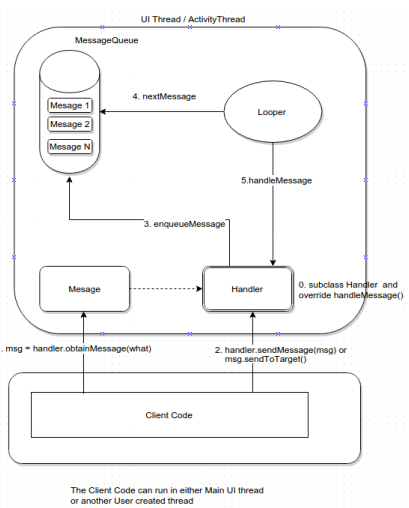
\includegraphics[scale=0.7]{Screenshot_2018-10-22_14-04-33.png}

\end{multicols}

\subsection{Splitting threads}
\begin{itemize}
\item Long (ish) running code that does not involve the UI
\begin{itemize}
  \item E.g. an image download 
  \item Occurs in a separate thread of execution
  \item Still tightly coupled to an activity
  \item Not allowed to do network communication in the UI thread
\end{itemize}
\item Instantaneous code that does involve the UI
\begin{itemize}
  \item E.g. drawing the image that has been downloaded
  \item posted to the UI thread responsible for a particular View to execute, logically parceled up as a Runnable object
  \item Risk of orphaned threads
\end{itemize}
\end{itemize}

\section{AsyncTask}
\begin{flushleft}
A convenience class for making complex asynchronous worker tasks easier. Worker / blocking tasks are executed in a background thread.
Can get data back using \textbf{results callback}, and it's executed in the UI thread. With each AsyncTask that is spun off, a thread is created and destroyed, which might be a performance issue. We can solve this by implementing implement a thread pool.
\end{flushleft}

\section{Services}
\begin{flushleft}
An	Application	Component	that
\begin{itemize}
  \item Has	no	UI
  \item Represents	a	desire	to	perform	a	longer-running	operation. I.e.	longer	than	a	single-activity	element	of	the	task
  \item Threads	are	associated	with	the	activity	that	started	them i.e.	could	be orphaned
\end{itemize}
Activities	are	loaded/unloaded	as	users	move	around	app, where as services	\textbf{remain	for	as	long	as	they	are	needed}.
Can expose	functionality	for	other	apps: one	service	\textbf{may	be	used	by	many	applications}, which allows to avoid	duplication	of	resources
\end{flushleft}


\subsection{What services are not}
\begin{itemize}
  \item Not a separate process
  \begin{itemize}
    \item Runs in the same process as the application in which it is declared (by default) 
  \end{itemize}
  \item Not a thread
  \begin{itemize}
    \item One thread per Application
    \item Handles events for all components
    \item If you need to do things in the background, start your own thread of execution
  \end{itemize}
\end{itemize}

\subsection{Uses of Services}
\begin{itemize}
  \item MP3	Playback: Want to play audio while the user is doing other things
  \item Network Access: long download, sending email, polling email server for new mail.
  \item Anything	that	you	don’t	want	to	interrupt	the	user	experience	for
\end{itemize}

\subsection{Creating a Service}
Services	are	designed	to	support	communication	with
\begin{itemize}
  \item Local	Activities	(in	the	same	process). For example: within	VM
  \item Remote	Activities	(in	a	different	process). For example IPC
  \item Multiple	components
  \begin{itemize}
    \item System services	underpin	much	of	Android	core	OS,	but	wrapped	with	various	APIs
  \end{itemize}
\end{itemize}

\newpage

\section*{Reference section} \label{sec:reference}
\begin{description}
	\item[atomic] \hfill \\ Something that "appears to the rest of the system to occur instantaneously" (One operation at a time).\textbf{Atomic operation} means an operation that appears to be instantaneous from the perspective of all other threads. You don't need to worry about a partly complete operation when the guarantee applies.
\end{description}
\end{document}
